\chapter{Bestimmung der IQE bei Raumtemperatur}
\thispagestyle{fancy}

In diesem Kapitel wird die in Kapitel vorgestellte Methode zur Bestimmung der IQE bei Raumtemperatur benutzt und versucht auf eine möglichst große Anzahl von uns gemessenen Proben anzuwenden. 
Um dies generisch und automatisiert zu verwirklichen und die Methode auf möglichst viele und auch alte Messungen anzuwenden, wurde von mir ein Mathematica-Skript geschrieben, dass die gemessenen Daten einer Probenserie bei Raumtemperatur benutzt, um die Ergebnisse in Echtzeit in Abhängigkeit von einem variablen Bereich der Messpunkte darzustellen. Dies erscheint wichtig, weil die Methode das ABC-Modell auf die Parameter A und B reduziert und somit möglichst ein Bereich ausgewählt werden sollte, bei dem der Einfluss der Auger-Rekombination gering ausfällt. Also muss insbesondere der Bereich geringer Anregungsleistungsdichten betrachtet werden, der allerdings mit unserem UVPL-Setup stark von Messartefakten und Rauschen beeinflusst ist. So zeigte sich, dass die Methode für keine Probenserie verlässliche Werte lieferte und stattdessen die Ergebnisse stark mit dem ausgewählten Bereich der Datenpunkte variierte und das so sehr, dass die Methode für die Bestimmung der IQE unserer Proben als unbrauchbar beschrieben werden muss. Die große Schwankung in Abhängigkeit der ausgewählten Datenpunkte ist in Abbildung \ref{fig:raumtemp} zu sehen. Dieses Verhalten mit der starken Schwankung wiesen alle untersuchten Proben auf. 
%
\begin{figure}[H]
\begin{tabular}{ccc}
  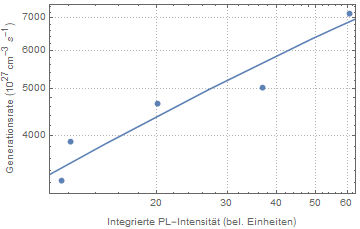
\includegraphics[width=0.30\textwidth]{Bilder/RaumtempBilder/genfit1-5.png} & 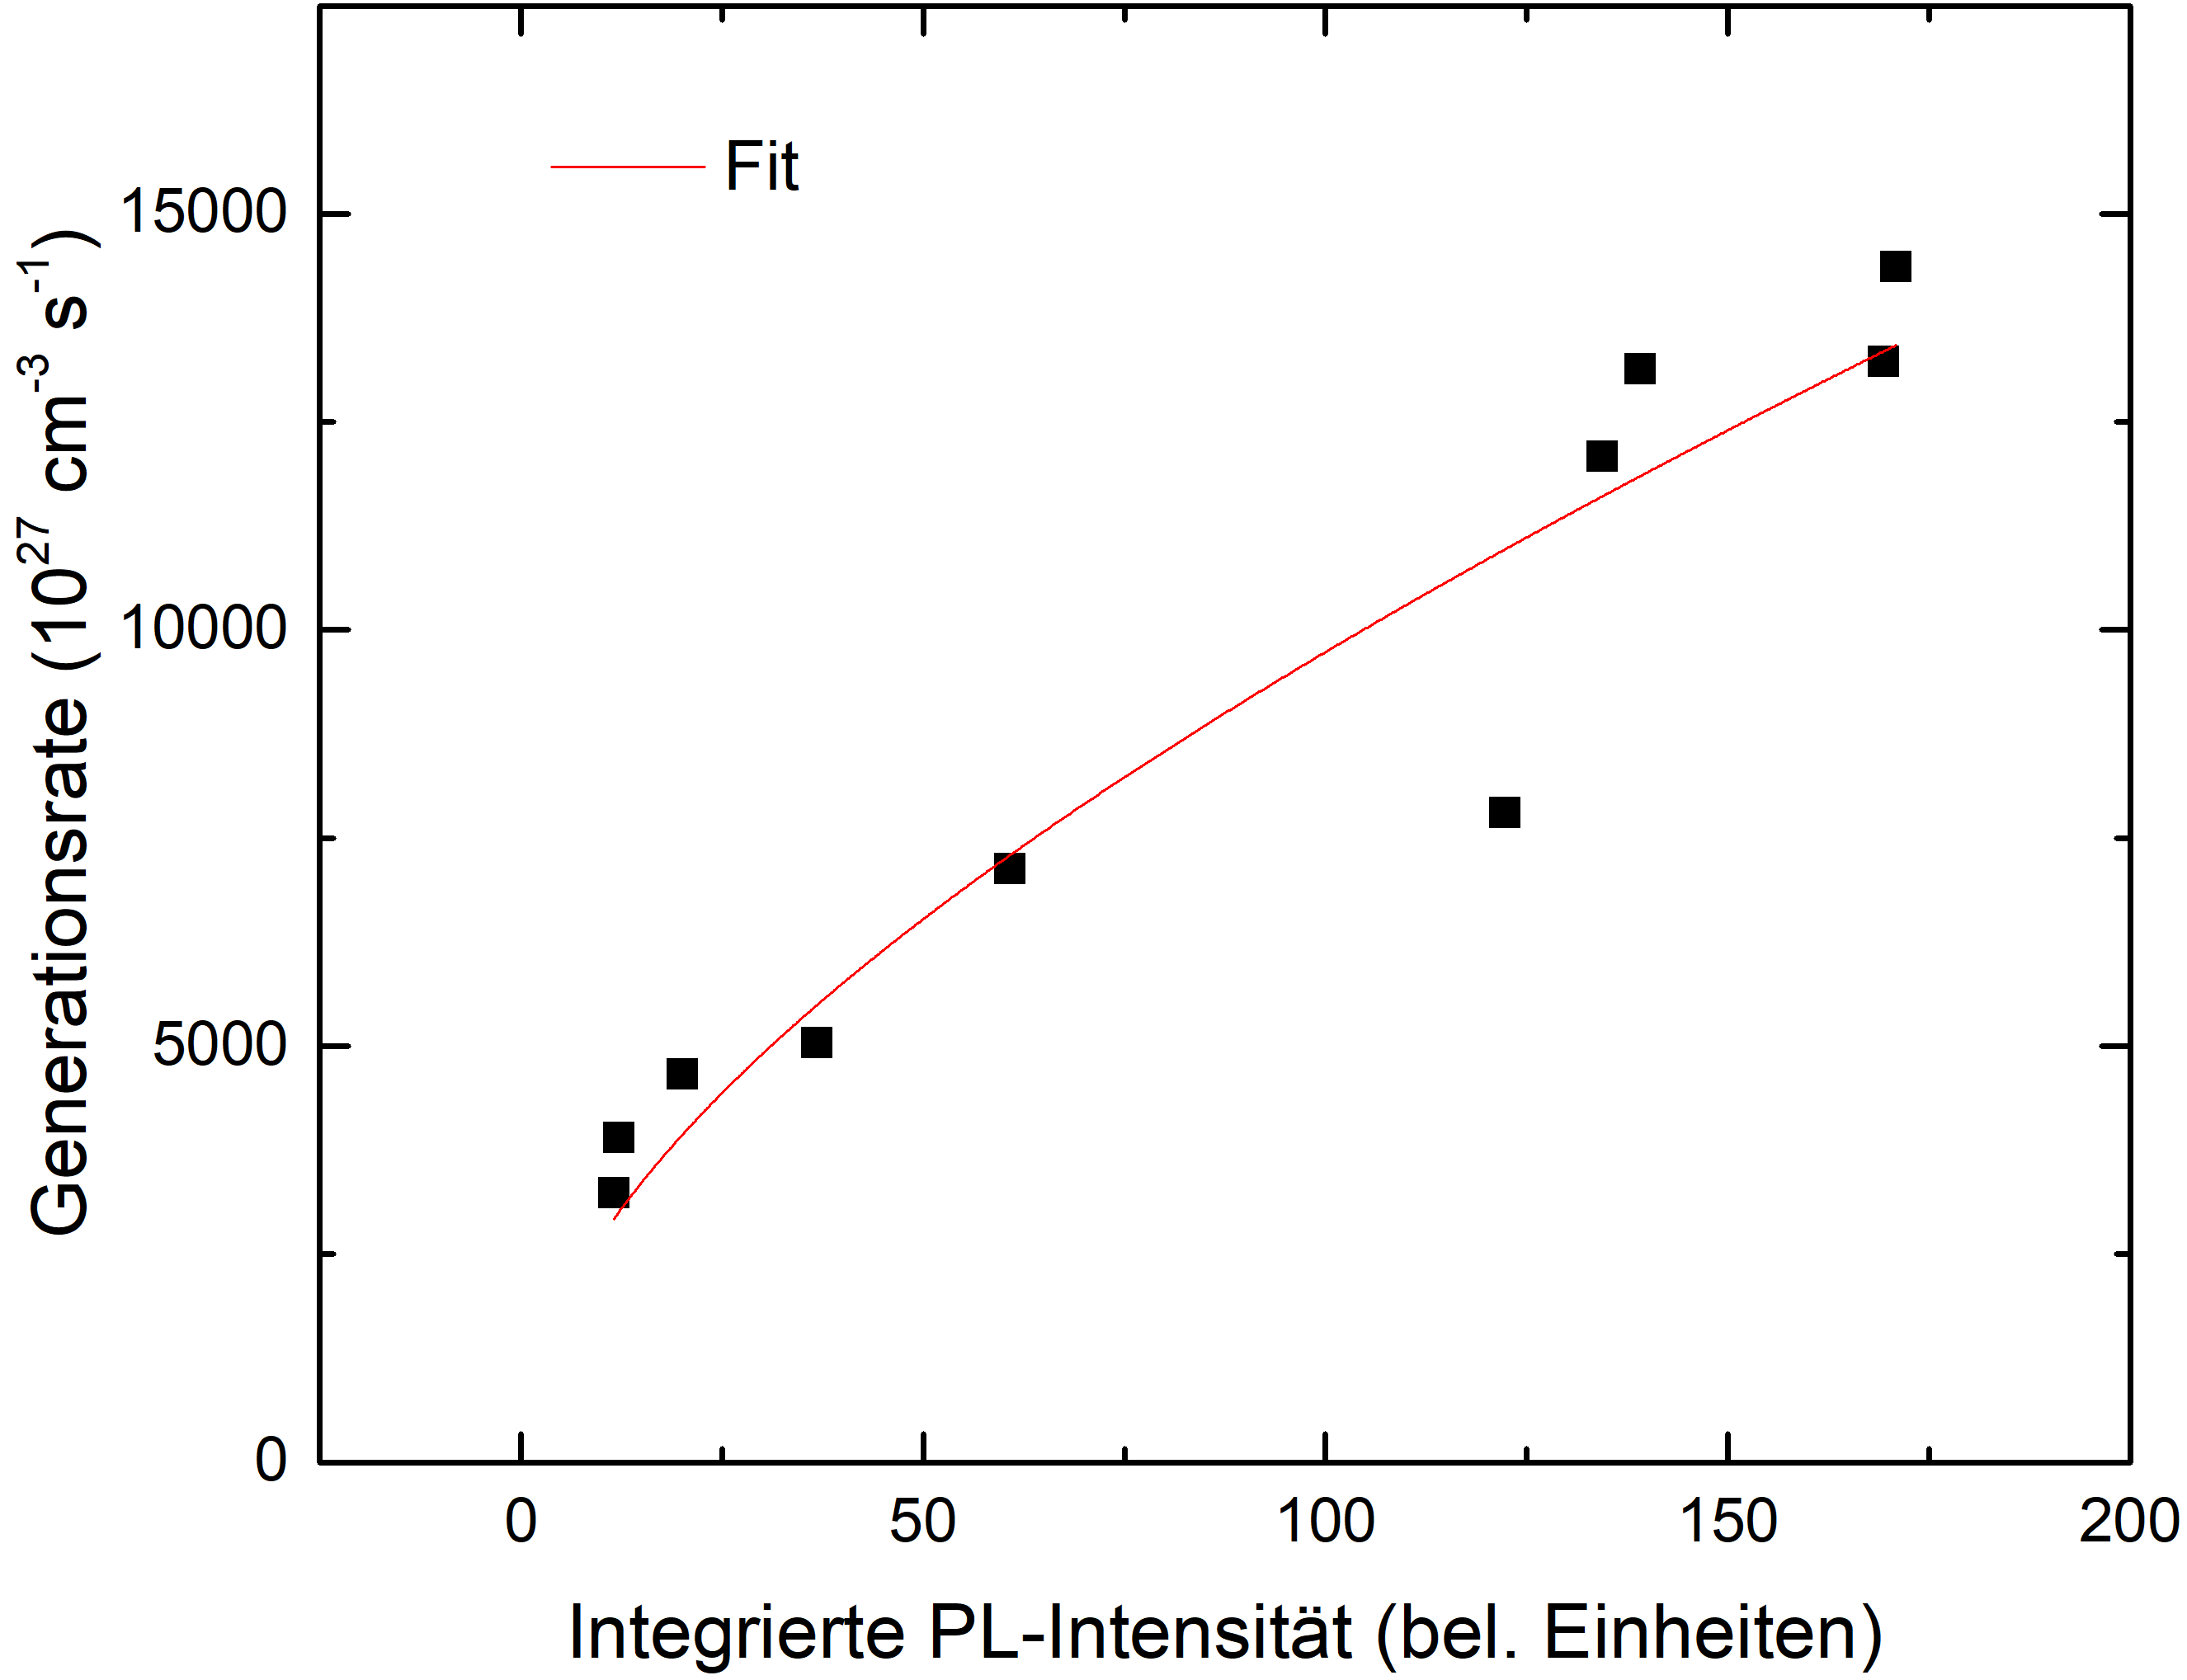
\includegraphics[width=0.32\textwidth]{Bilder/RaumtempBilder/genfit1-10.png}  & 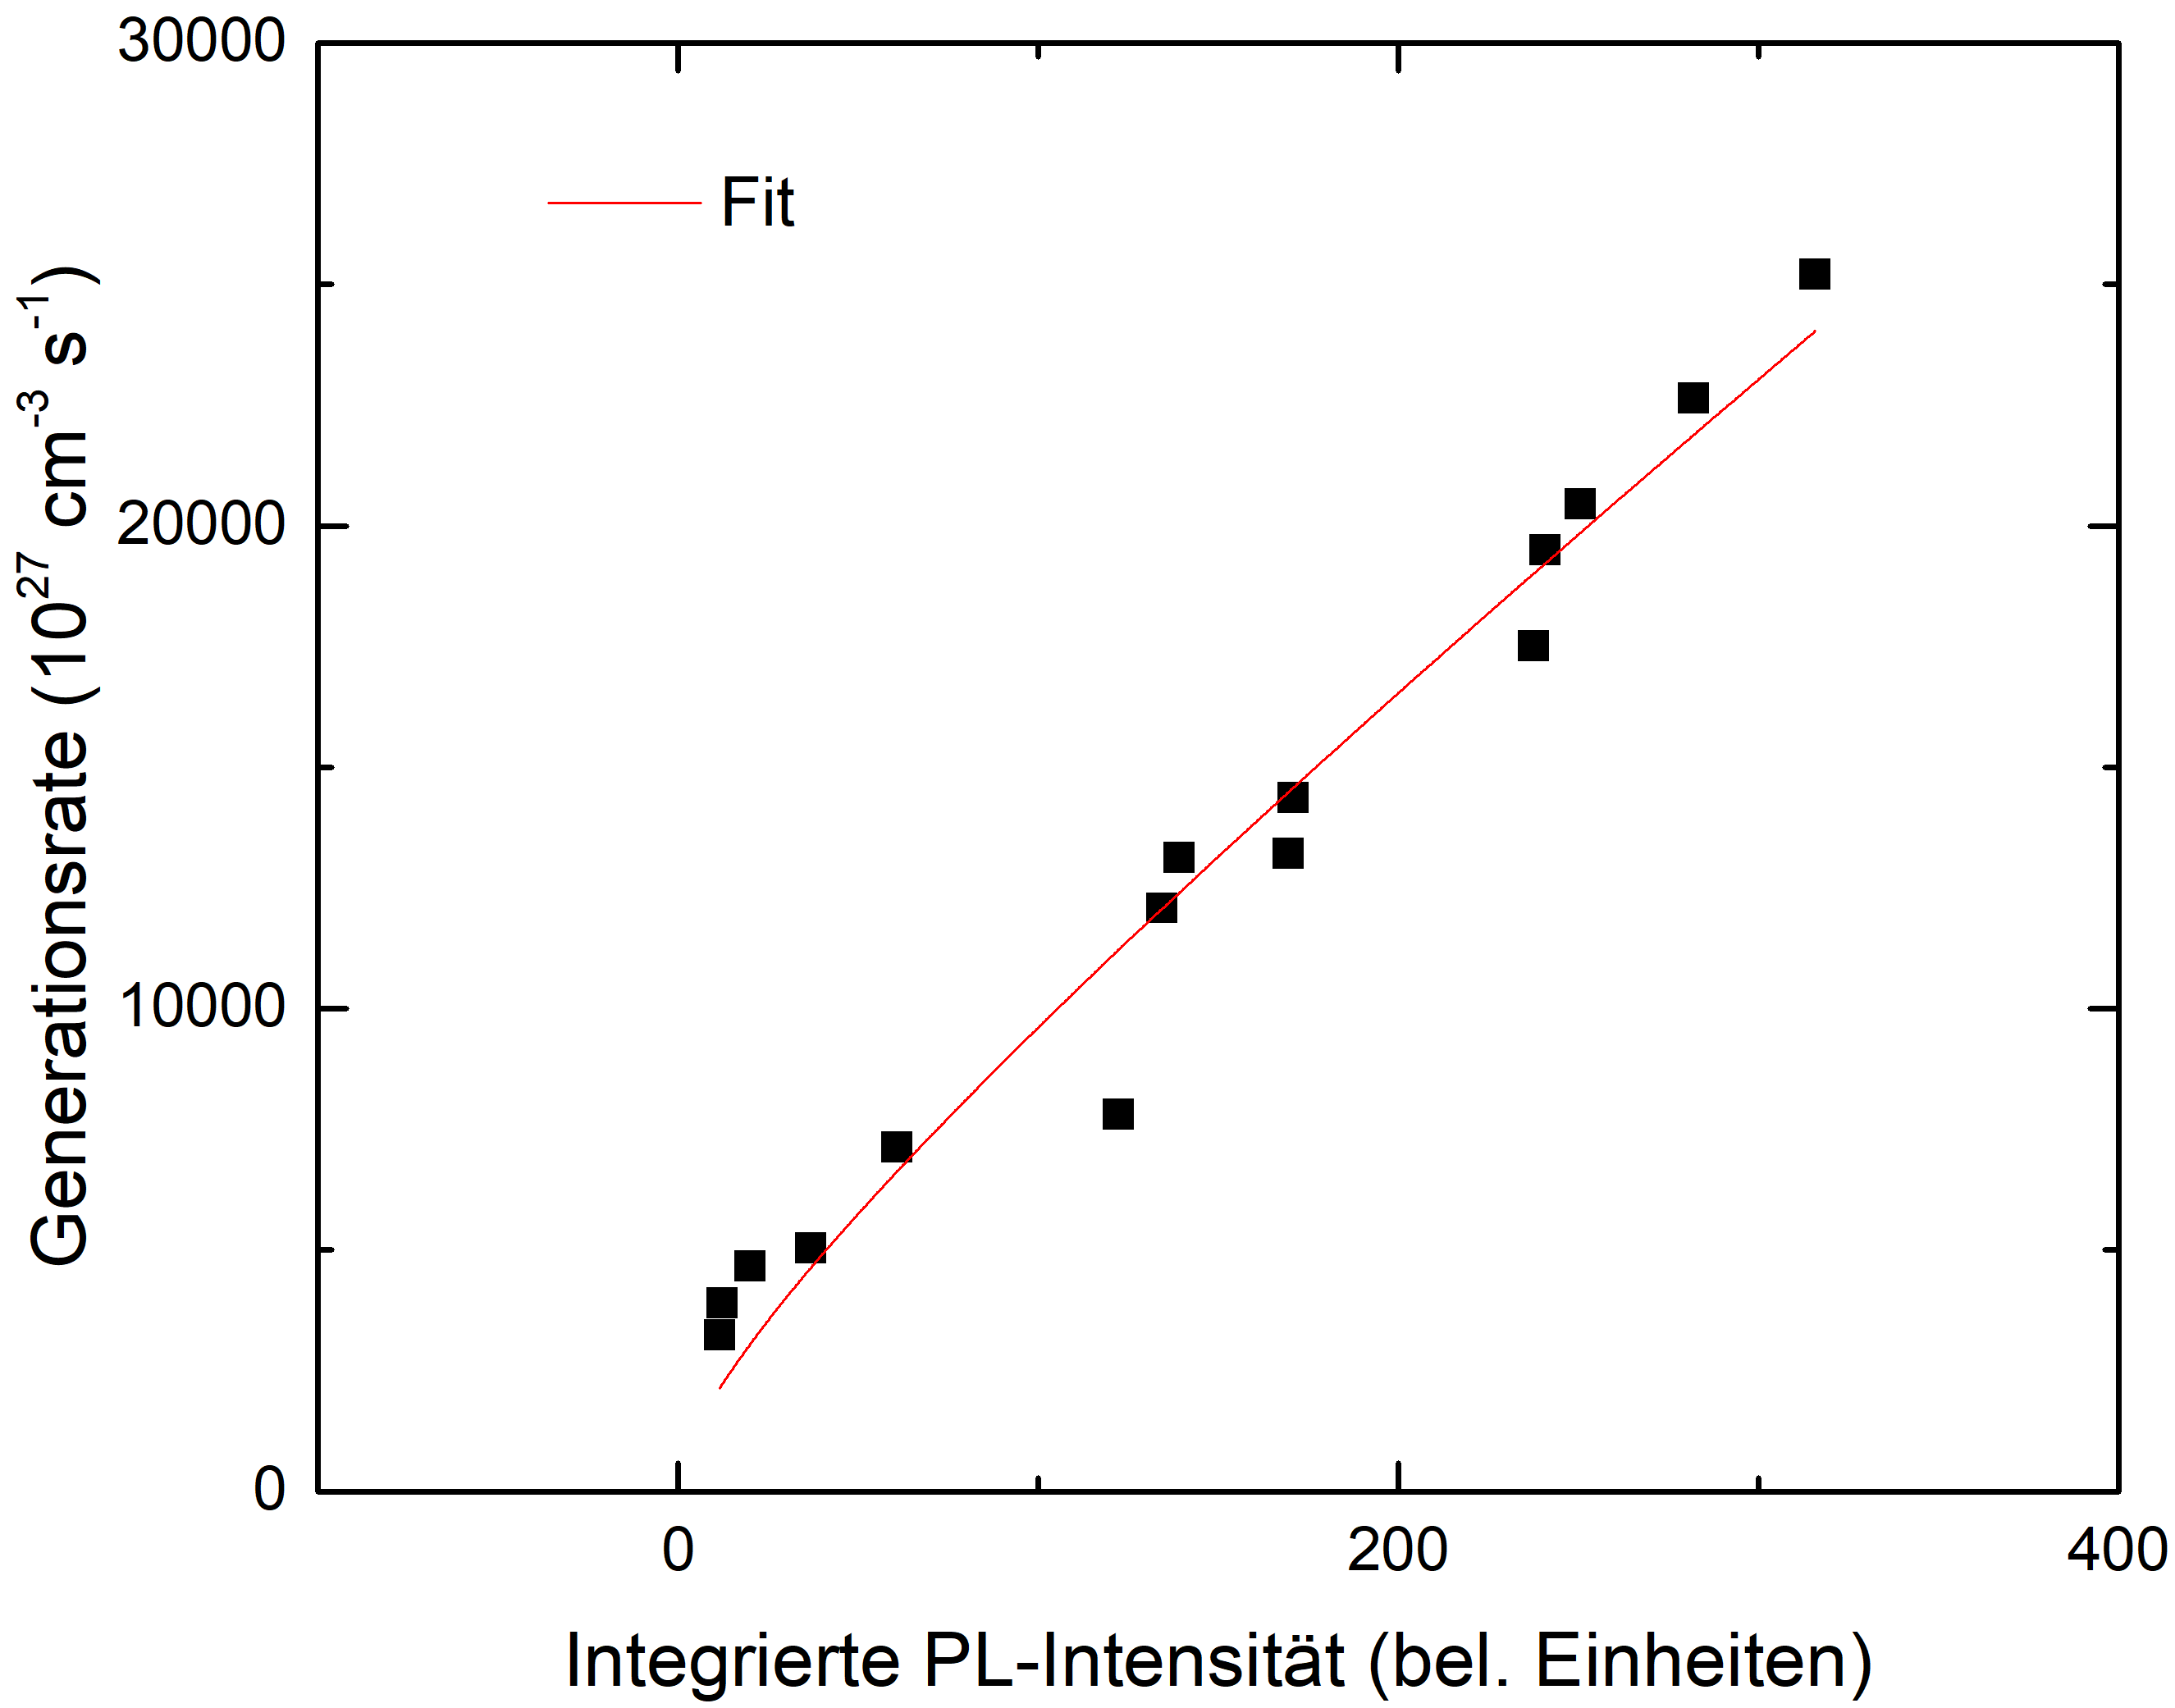
\includegraphics[width=0.30\textwidth]{Bilder/RaumtempBilder/genfit1-15.png} \\
 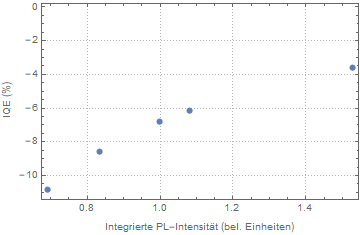
\includegraphics[width=0.30\textwidth]{Bilder/RaumtempBilder/iqe1-5.png} &   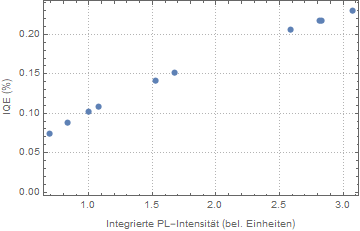
\includegraphics[width=0.30\textwidth]{Bilder/RaumtempBilder/iqe1-10.png} & 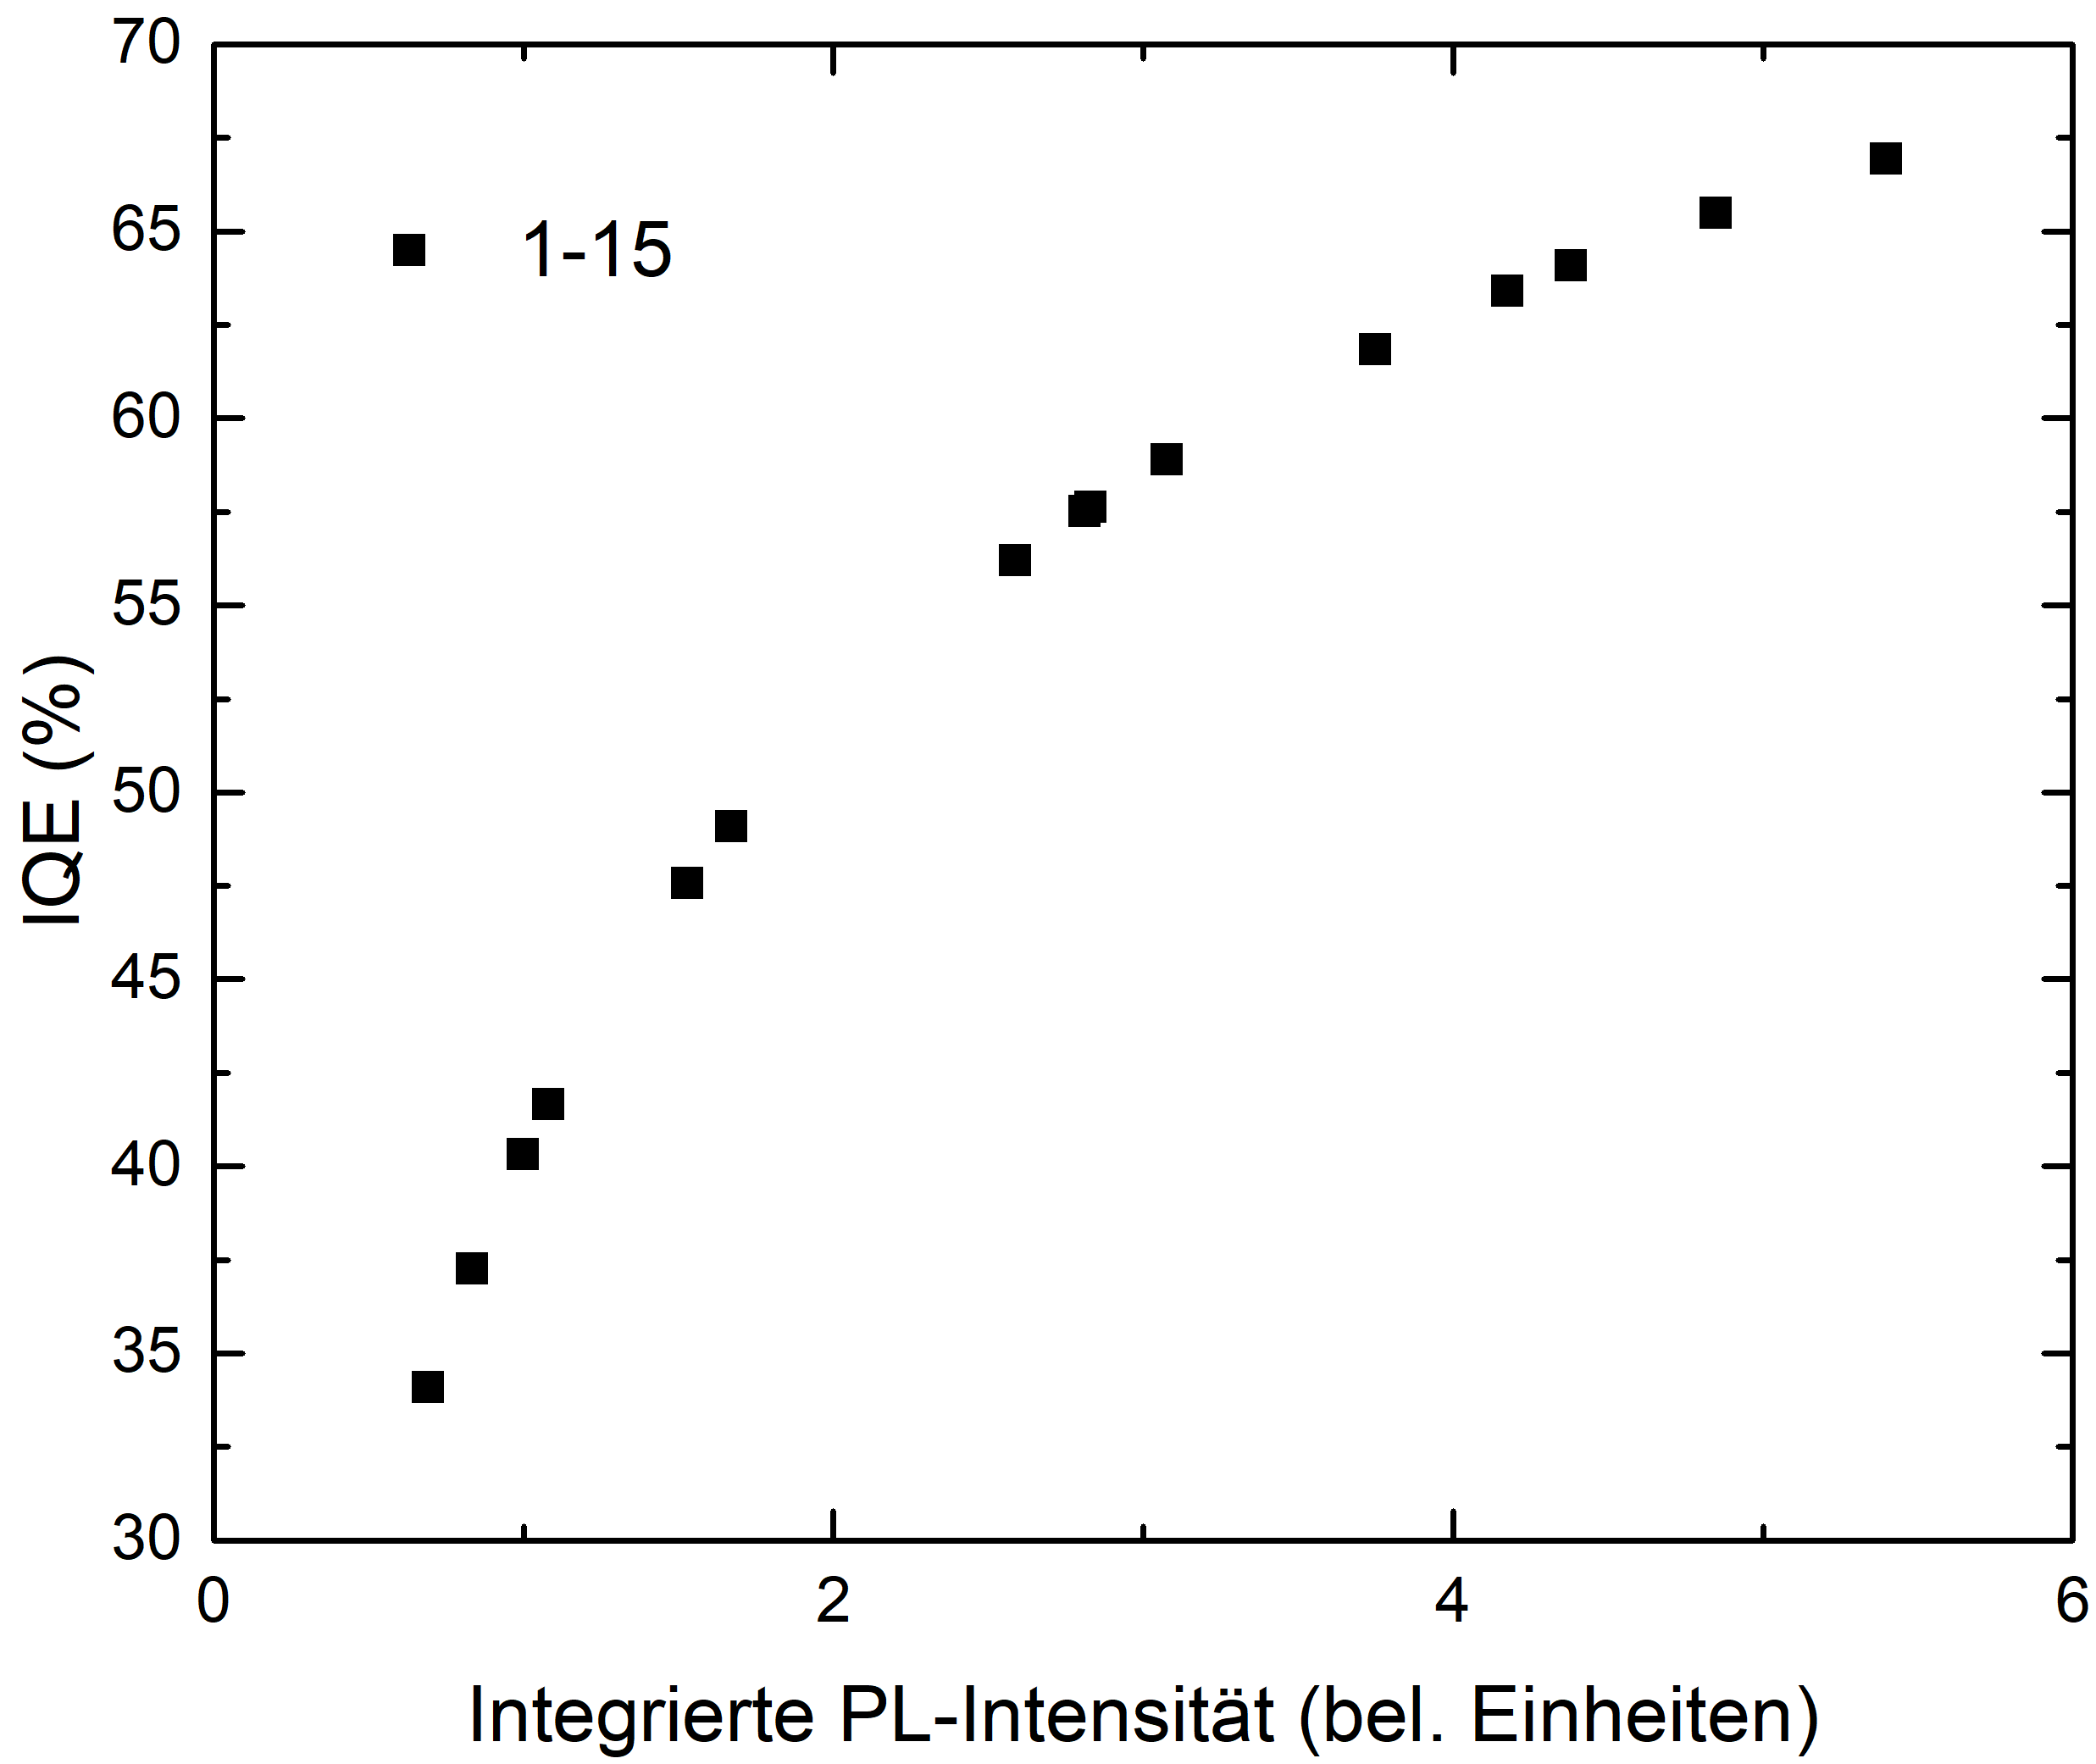
\includegraphics[width=0.30\textwidth]{Bilder/RaumtempBilder/iqe1-15.png}  \\
 a & b & c
\end{tabular}
\caption{Der Fit der Generationsrate in Abhängigkeit der integrierten Intensität für die 1-5 (a), 1-10 (b) und 1-15 (c) Datenpunkte und darunter die aus dem Fit bestimmte IQE.}
\label{fig:raumtemp}
\end{figure}
\noindent 
Des Weiteren sollte erwähnt werden, dass die zugehörigen A- und B-Parameter in keinem der Fälle in einem Bereich lag, in dem sie nach Literaturwerten einzuordnen wären. Stattdessen schwankten sie variierend mit einigen Zehnerpotenzen darüber oder darunter. 
Nun soll auf die Problematik des Ansatzes der angewandten Methode eingegangen werden. 

%Bei Proben mit Laserstruktur (erste und letzte Barriere des MQWs sind Waveguides) fiel insbesondere auf, dass die Form der Kurve von der des Fits besonders stark abweicht und wahrscheinlich bedingt ist, durch die komplexere Struktur im Vergleich zu normalen LED-Strukturen. 

